\lab{Linear Transformations}{Linear Transformations}
% \objective{Apply affine transformations to a set of vectors in $\mathbb{R}^2$.}
% \objective{Introduce the temporal and spatial complexity and explore SciPy's methods for working with sparse matrices.}

\section*{Numerical Linear Operations} % ======================================

\subsection*{Timing Code} % ---------------------------------------------------

The \li{time} module includes functions that access for dealing with time.
This is useful for precisely measuring how long it takes for code to run.
The \li{time()} function in the \li{time} module measures the number of seconds from a fixed starting point, the ``Epoch.''
For most machines, this starting point will be January 1, 1970.

\begin{lstlisting}
>>> import time

>>> time.time()
1436832057.321525
\end{lstlisting}

In order to measure how long it takes to execute some Python code, record the time just before and just after the code in question.
Subtracting the first measurement from the second gives the amount of time in seconds that have passed.

\begin{lstlisting}
# Time how long it takes to go through 10000 iterations using 'range'.
>>> def time_for_loop():
...     start = time.time()         # Clock the starting time.
...     for i in range(10000):      # Perform the operation.
...         pass
...     end = time.time()           # Clock the ending time.
...     return end - start          # Report the difference.
\end{lstlisting}

The standard library also has a module called \li{timeit}.
This library is built specifically to time Python code and has more sophisticated tools than the \li{time} module.
In IPython, \li{timeit} can be used like a built-in function any time with the \li{\%timeit} command.

\begin{lstlisting}
# Time how long it takes to go through 10000 iterations using 'xrange'.
In [0]: %timeit for i in xrange(10000): pass 
1000 loops, best of 3: 303 µs per loop
\end{lstlisting}

\begin{comment} % Old problem. Can this be rehashed somehow?
\begin{problem}
Download \texttt{matrix\_multiply.py} and \texttt{matrices.npz}.
The Python file \texttt{matrix\_multiply.py} is a module that has three functions for multiplying two matrices together, called \li{method1()}, \li{method2()}, and \li{method3()}.
It also has a \li{load\_matrices()} function that returns two matrices from \texttt{matrices.npz}.

Modify your solutions file so that when it is run from a Python interpreter (but not when it is imported), the following is executed:
\begin{enumerate}
\item If no command line arguments are given, print ``No Input."
\item If anything other than ``matrices.npz'' is given, print ``Incorrect Input."
\item If ``matrices.npz'' is given as a command line argument, load two matrices from \texttt{matrices.npz}. Time (separately) how long each method takes to multiply the two matrices together, then print the results.

(Hint: Read the code in \texttt{matrix\_multiply.py}, especially the function docstrings, to determine how to use each function.)
\end{enumerate}
\end{problem}
\end{comment}

\subsection*{Matrix-Vector Multiplication} % ----------------------------------

\subsection*{Matrix-Matrix Multiplication} % ----------------------------------

\subsection*{Why NumPy} % -----------------------------------------------------

% The coefficient for list of lists is way bigger than it is with NumPy arrays.

\begin{lstlisting}
In [1]: import numpy as np
In [2]: from random import random

# Make two lists of 10000 random entries and corresponding NumPy arrays.
In [3]: a = [random() for i in xrange(10000)]
In [4]: b = [random() for i in xrange(10000)]
In [5]: A, B = np.array(a), np.array(b)

In [6]: %timeit [x + y for x,y in zip(a,b)]
100 loops, best of 3: 2.02 milisecons per loop          # .00202 seconds.

In [7]: %timeit A + B
100000 loops, best of 3: 92.9 microseconds per loop     # .0000929 seconds.
\end{lstlisting}

Apart from being syntactically convenient, element-wise NumPy operations are also significantly faster than element-wise list operations.

\begin{lstlisting}
>>> from time import time
>>> from random import random

# Make two random lists with 10000 entries each.
>>> a = [random() for i in xrange(10000)]
>>> b = [random() for i in xrange(10000)]

# Time the element-wise addition for lists.
>>> start = time()
>>> [x + y for x, y in zip(a, b))]
>>> list_time = time() - start

# Cast each list as a NumPy array.
>>> A, B = np.array(a), np.array(b)

# Time the element-wise addition for arrays.
>>> start = time()
>>> a + b
>>> array_time = time() - start

# Report the times.
>>> print list_time, array_time
0.0030951499939 0.000310897827148
\end{lstlisting}

\begin{problem} % Time matrix multiplication.
For a $m\times n$ matrix $A$ with entries $a_{ij}$ and an $n\times l$ matrix $B$ with entries $b_{ij}$, the matrix product $C = AB$ is defined entrywise by the formula:
\[c_{ij} = \sum_{k=1}^N a_{ik}b_{kj}\]

The following function performs matrix multiplication using nested lists without using NumPy.

\begin{lstlisting}
def matrix_multiply(A, B):
    """Calculate the matrix product AB.
    Each parameter is a list of lists.
    """
    # Get the dimensions of the matrices and initialize the new 'matrix'.
    m, n, l = len(A), len(B), len(B[0])
    result = []

    # Calculate each entry of the new matrix.
    for i in range(m):
        for j in range(l):
            result.append(sum([A[i][k] * B[k][j] for k in xrange(n)]))
    return result
\end{lstlisting}

Write a function that times matrix multiplication with the above function, and compare it with numpy.dot().
A random matrix $1000\times 1000$ as a list of lists can be created with

\begin{lstlisting}
a = [[random() for j in xrange(1000)] for i in xrange(1000)]
\end{lstlisting}

\end{problem}

Iterating through this triple \li{for} loop is very expensive.
NumPy also uses loops, but it uses C loops instead of Python loops.
Compare the difference between the pure Python and the NumPy ways:

\begin{lstlisting}
def arr_mult(A,B):
    # return [[ sum([A[i][k] * B[k][j] for k in xrange(len(B))   ]) 
    #                                  for j in xrange(len(B[0])) ]
    #                                  for i in xrange(len(A))    ]
    matrix = []
    # Iterate over the rows of A.
    for i in range(len(A)):
        # Create a new row to insert into the product.
        row = []
        # Iterate over the columns of B.
        for j in range(len(B[0])):
            # Initialize an empty total.
            total = 0
            # Multiply the elements of the row of A with 
            # the column of B and sum the products.
            for k in range(len(B)):
                total += A[i][k] * B[k][j]
            # Insert the value into the new row of the product. 
            row.append(total)
        # Insert the new row into the product.
        matrix.append(row)
    return matrix
\end{lstlisting}

Table \ref{table:square_times} documents how long\footnote{You can replicate this experiment yourself. In IPython, you can find the execution time of a line of code by prefacing it with \li{\%timeit}.
If you aren't using IPython, you will need
to use the timeit function documented here: \url{https://docs.python.org/2/library/timeit.html}.}
one computer took to square a $k \times k$ matrix in both Python (using the function \li{arr_mult}) and NumPy (using the method you found in Problem \ref{prob:simple1}) for various values of $k$.
As you can see, NumPy is much faster.
One reason for this is that algorithms in NumPy are usually implemented in C or in Fortran.

\begin{table}
 \begin{tabular}{|c|l|l|} \hline Data Structure & $k\times k$ & Time (s) \\ \hline
 Python List    & $10\times10$  & 0.0002758503 \\
 \cline{2-3}    & $100\times100$    & 0.1336028576 \\
 \cline{2-3}    & $1000\times1000$ & 200.4009799957 \\
 %& $1\times1$      & 0.0000181198 \\
\hline \hline
 NumPy Array    & $10\times10$  & 0.0000109673 \\
 \cline{2-3}    & $100\times100$    & 0.0009210110 \\
 \cline{2-3}    & $1000\times1000$ & 2.1682999134 \\
 %& $1\times1$      & 0.0000298023 \\
 \hline \end{tabular}
 \caption{Time for one computer to square a $k \times k$ matrix in Python and NumPy.}
\label{table:square_times}
\end{table}
%
NumPy is optimized for fast array computations.

% Note about Caching.

\section*{Linear Transformations} % ===========================================

% Definition of a Linear Transformation.

\subsection*{Dilations}
A \emph{dilation} of the vector space rescales the vectors. 
Graphically, a dilation stretches or compresses the space. 
A linear transformation is a dilation if and only if its matrix representation is diagonal, so in particular all Type II elementary matrices are dilations. 
The matrix $\begin{pmatrix}
1.5 & 0\\
0 & 1.5 \end{pmatrix}$ corresponds to the dilation in Figure \ref{fig:dilation}.
\begin{figure}
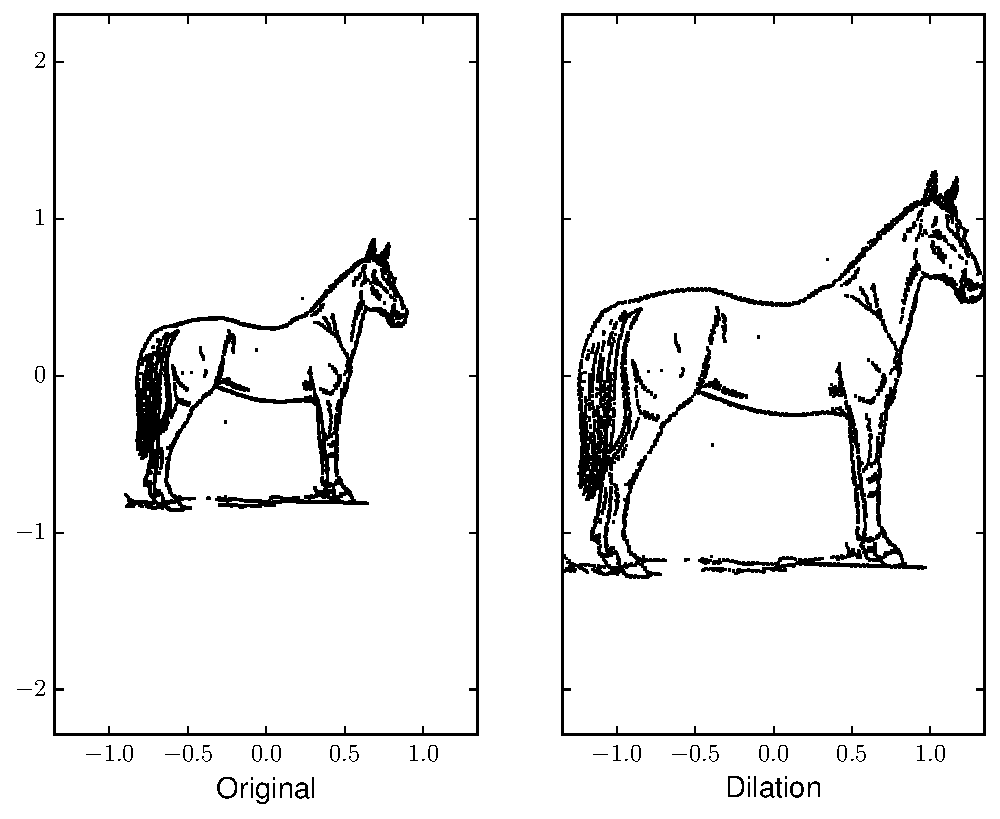
\includegraphics[width=\textwidth]{stretch.pdf}
\caption{An example of a dilation. 
The image on the left was stretched by a factor of $1.5$ in all directions, producing the image on the right.}
\label{fig:dilation}
\end{figure}

\begin{problem}\label{prob:dilation}
Write a function that accepts an array of points and an array giving the stretching factors in each direction. 
Your function should return the dilated points. 
Hint: To check your work, plot the original points and their images under the transformation using the function \li{plotOldNew()} defined below.
\begin{lstlisting}
import numpy as np
from matplotlib import pyplot as plt

def plotOldNew(old, new):
    '''Inputs:
    new -- a (2,n) numpy array containing x-coordinates on the 
            first row and y-coordinates on the second row.
    old -- a (2,n) numpy array containing x-coordinates on the first
            row and y-coordinates on the second row.
    '''
            
    plt.subplot(2, 1, 1)
    plt.scatter(old[0], old[1])
    plt.axis('equal')
    plt.subplot(2, 1, 2)
    plt.scatter(new[0], new[1])
    plt.show()
\end{lstlisting}
\end{problem}

\subsection*{Rotations} % -----------------------------------------------------

A second type of linear transformation is to rotate vectors around the origin. 
A rotation of $\theta$ radians counterclockwise corresponds to the matrix $\begin{pmatrix}
\cos(\theta) & -\sin(\theta) \\
\sin(\theta) & \cos(\theta)
\end{pmatrix}.$ 
When $\theta = \pi/3$ we get the rotation matrix illustrated in Figure \ref{fig:rotate}.

\begin{figure}
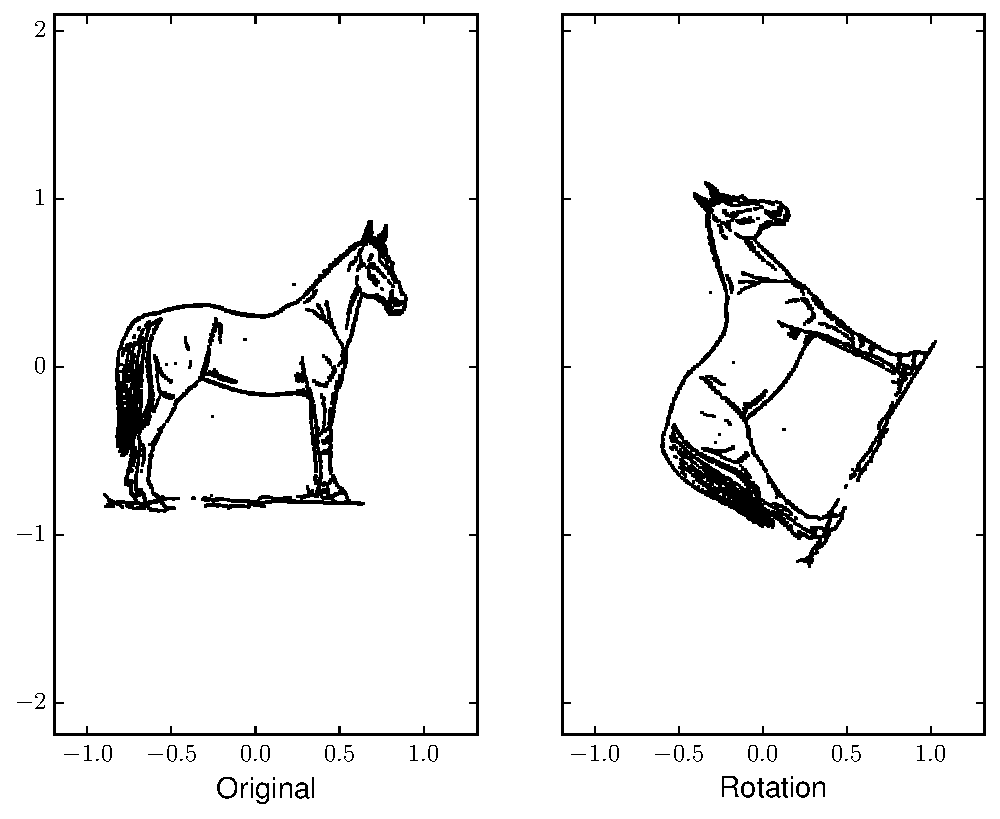
\includegraphics[width=\textwidth]{rotate.pdf}
\caption{An example of a rotation.
The image on the left was rotated by $\pi/3$, producing the image on the right.}
\label{fig:rotate}
\end{figure}

\begin{problem}
 Write a function that accepts an array of points and the angle of rotation (in radians). 
 Your function should return the rotated points. 
 Hint: To check your work, plot the original points and their images under the transformation using the function \li{plotOldNew()} defined in Problem \ref{prob:dilation}.
\end{problem}

\subsection*{Shears} % --------------------------------------------------------

\begin{figure}
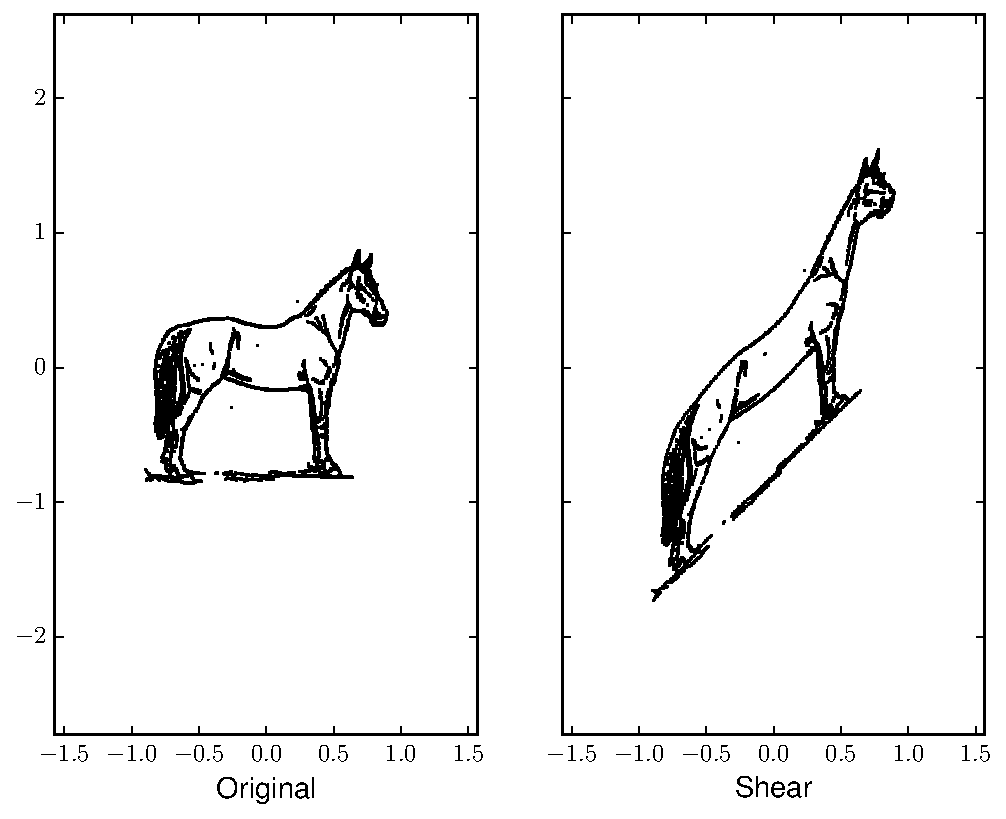
\includegraphics[width=\textwidth]{shear.pdf}
\caption{An example of a shear.
The image on the right was sheared vertically to produce the image on the left.}
\label{fig:shear}
\end{figure}

A third type of linear transformation is a \emph{shear}, which ``slants'' a set of vectors. 
The corresponding matrix is a Type III elementary matrix. 
A horizontal shear has the form $\begin{pmatrix}
1 & c \\
0 & 1
\end{pmatrix}$ and a vertical skew has the form $
 \begin{pmatrix}
1 & 0 \\
c & 1
\end{pmatrix}
$. 
Notice that horizontal skews fix the $y$-coordinate of a vector while vertical skews fix the $x$-coordinate. 
The horizontal shear in Figure \ref{fig:shear} corresponds to the matrix $\begin{pmatrix}
1 & 1.02 \\
0 & 1
\end{pmatrix}
$.


\begin{problem}
Write a function that accepts an array of points, a floating point argument that indicates the shearing amount, and an integer argument that indicates the direction of the shear (0 for horizontal, 1 for vertical). 
Your function should return the sheared points. 
Hint: To check your work, plot the original points and their images under the transformation using the function \li{plotOldNew()} defined in Problem \ref{prob:dilation}.
\end{problem}

\subsection*{Reflections}% ----------------------------------------------------

\begin{figure}
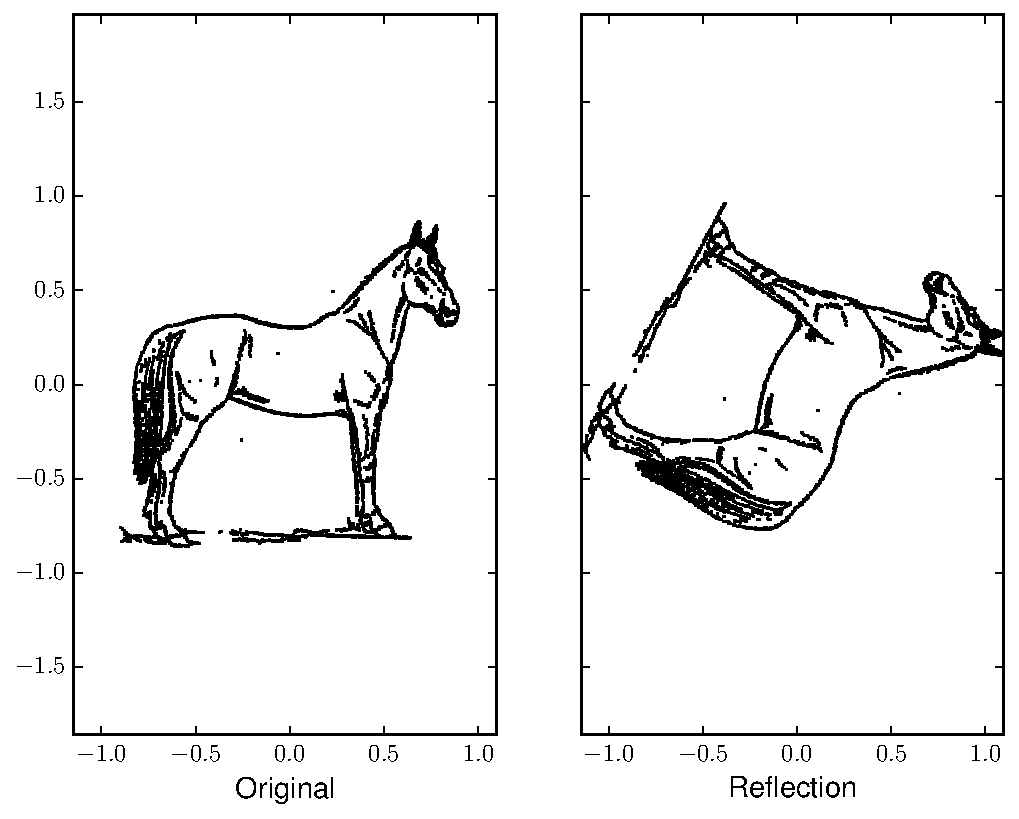
\includegraphics[width=\textwidth]{reflect.pdf}
\caption{An example of a reflection. 
The top image was reflected about the line $y = (1/\sqrt{3})x$, producing the bottom image.}
\label{fig:reflect}
\end{figure}
A fourth type of linear transformation is reflections about a line, also called \emph{Householder transformations}. 
Reflecting about a line spanned by $(l_1, l_2)$ corresponds to the matrix
\[
\frac{1}{l_1^2 + l_2^2}
\begin{pmatrix}
l_1^2 - l_2^2 & 2l_1l_2 \\
2l_1l_2 & l_2^2 - l_1^2
\end{pmatrix}.
\]

For example, the line $y=x$ is spanned by $(1, 1)$. 
In this case the corresponding matrix $\begin{pmatrix}
0 & 1\\
1 & 0
\end{pmatrix}$ is a Type I elementary matrix, in fact the only one of size $2 \times 2$. 
As another example, the reflection in Figure \ref{fig:reflection} about the line $y = (1/\sqrt{3})x$ corresponds to the matrix $\frac{1}{4}\begin{pmatrix}
2 & 2\sqrt{3}\\
2\sqrt{3} & -2
\end{pmatrix}$.

\begin{problem}
Write a function that accepts an array of points and a 1-D array describing the axis of reflection (in the notation above, this argument is $(l_1, l_2)$. 
Your function should return the reflected points. 
Hint: To check your work, plot the original points and their images under the transformation using the function \li{plotOldNew()} defined in Problem \ref{prob:dilation}.
\end{problem}

\subsection*{Composition of linear transformations}
Recall that composition of linear transformations corresponds to matrix multiplication. 
For example, if $S$ is a matrix representing a shear and $R$ is a matrix representing a rotation, then $RS$ represents a shear followed by a rotation.

In fact, any linear transformation of $\mathbb{R}^2$ is a composition of the transformations discussed in this lab. 
This is because reflections, dilations, and shears provide us with all the elementary matrices, and every matrix is a product of elementary matrices. 

\section*{Affine transformations}
\subsection*{Translations}

\begin{figure}
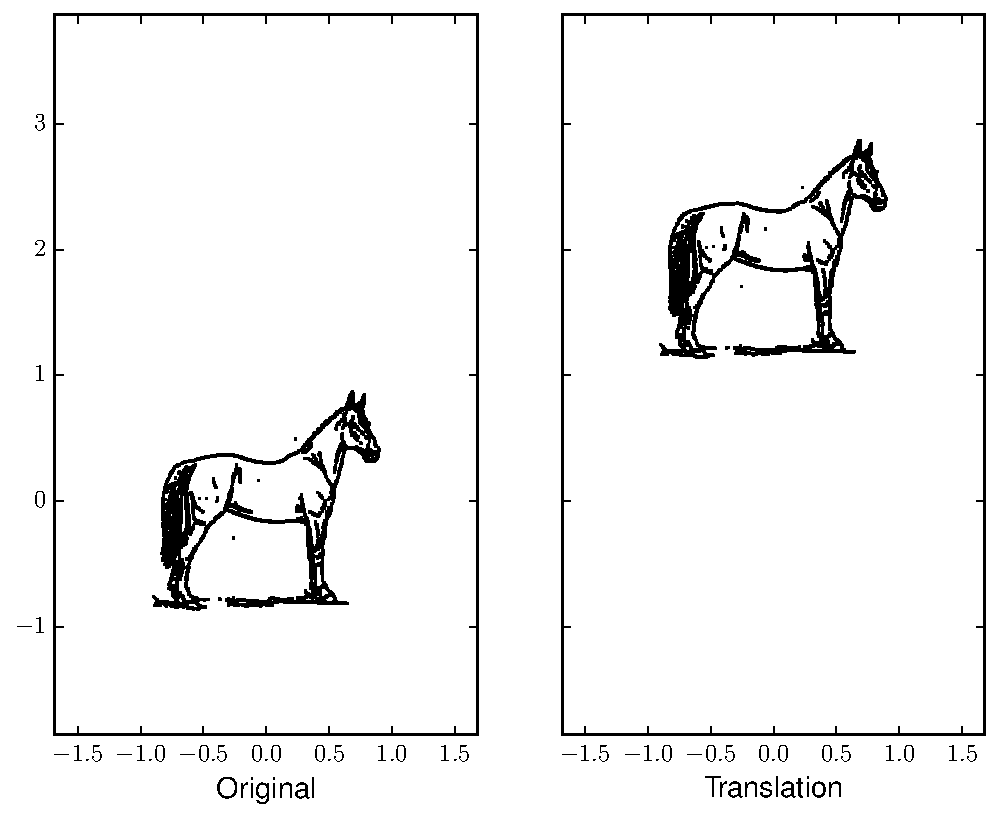
\includegraphics[width=\textwidth]{translate.pdf}
\caption{
An example of a translation.
The image on the left was translated by the vector $(0, 2)\trp$ to produce the image on the right.}
\label{fig:translation}
\end{figure}

A translation is a map $T: \mathbb{R}^2 \rightarrow \mathbb{R}^2$ defined by $T(\mathbf{x}) = \mathbf{x}+\mathbf{b}$ where $\mathbf{b} \in \mathbb{R}^2$. 
For example, if $\mathbf{b} = (2, 0)\trp$, then applying $T$ to an image will shift it right by 2. 
This translation is illustrated in Figure \ref{fig:translation}.


Translations are usually NOT linear maps. 
Therefore, they cannot be represented as matrix multiplication.

\begin{problem}
Write a function that accepts an array of points and an array indicating how much to shift them in each direction. 
The function should return the translated points. 
Hint: You can construct a $2 \times 1$ array using the syntax \li{np.array([[a], [b]])}. 
This may be more convenient for broadcasting. 
Another hint: To check your work, plot the original points and their images under the transformation using the function \li{plotOldNew()} defined in Problem \ref{prob:dilation}.
\end{problem}

\subsection*{Affine transformations}
Translations, together, with linear transformations, make up the broader class of transformations called ``affine transformations." 
These are transformations of the form $T: \mathbb{R}^2 \to \mathbb{R}^2$, $T(X) = AX + b$ where $A$ is an $n\times n$ matrix and $b \in \mathbb{R}^n$. 
Affine transformations include all compositions of scalings, rotations, dilations, reflections, and translations. 
For example, if $S$ represents a shear and $R$ a rotation, and if $\mathbf{b}$ is a vector in $\mathbb{R}^2$, then $T(\mathbf{x}) = RS\mathbf{x} + \mathbf{b}$ first shears $\mathbf{x}$, then rotates it, and finally translates it by $\mathbf{b}$. 


\begin{problem}
Imagine a particle $p_1$ rotating around a second particle $p_2$ which is moving through $\mathbb{R}^2$ in a straight line. 
Suppose $p_2$ begins at the origin and $p_1$ begins at $(1, 0)$. 
We can compute the trajectory of $p_1$ using affine transformations.

\begin{enumerate}\label{prob:trajectory}
\item Write a function that returns the position of $p_1$ at a time $t$. 
Your function should accept a time $t$, an angular velocity $\omega$, a direction vector $\mathbf{v}$, and a speed $s$. 
Assume $p_1$ rotates with angular velocity $\omega$ and $p_2$ moves in the direction of $\mathbf{v}$ with speed $s$.
The location of $p_1$ at time $t$ can be computed as follows:
\begin{itemize}
\item Calculate the position of $p_2$ at time $t$ with the formula $(st/\|\mathbf{v}\|) \mathbf{v}$.
\item Calculate the position of $p_1$ as follows:
\begin{itemize}
\item Rotate $p_1$ by $t\omega$ radians.
\item Translate the resulting vector by the vector equal to the position of $p_2$ at time $t$.
\end{itemize}
\end{itemize}
\end{enumerate}
\item Plot the trajectory of $p_1$ on the time interval $(0, 10)$ assuming $\omega=\pi$, $v=(1, 1)$, and $s=3$. 
Your graph should look something like Figure \ref{fig:trajectory}.
\begin{figure}[H]
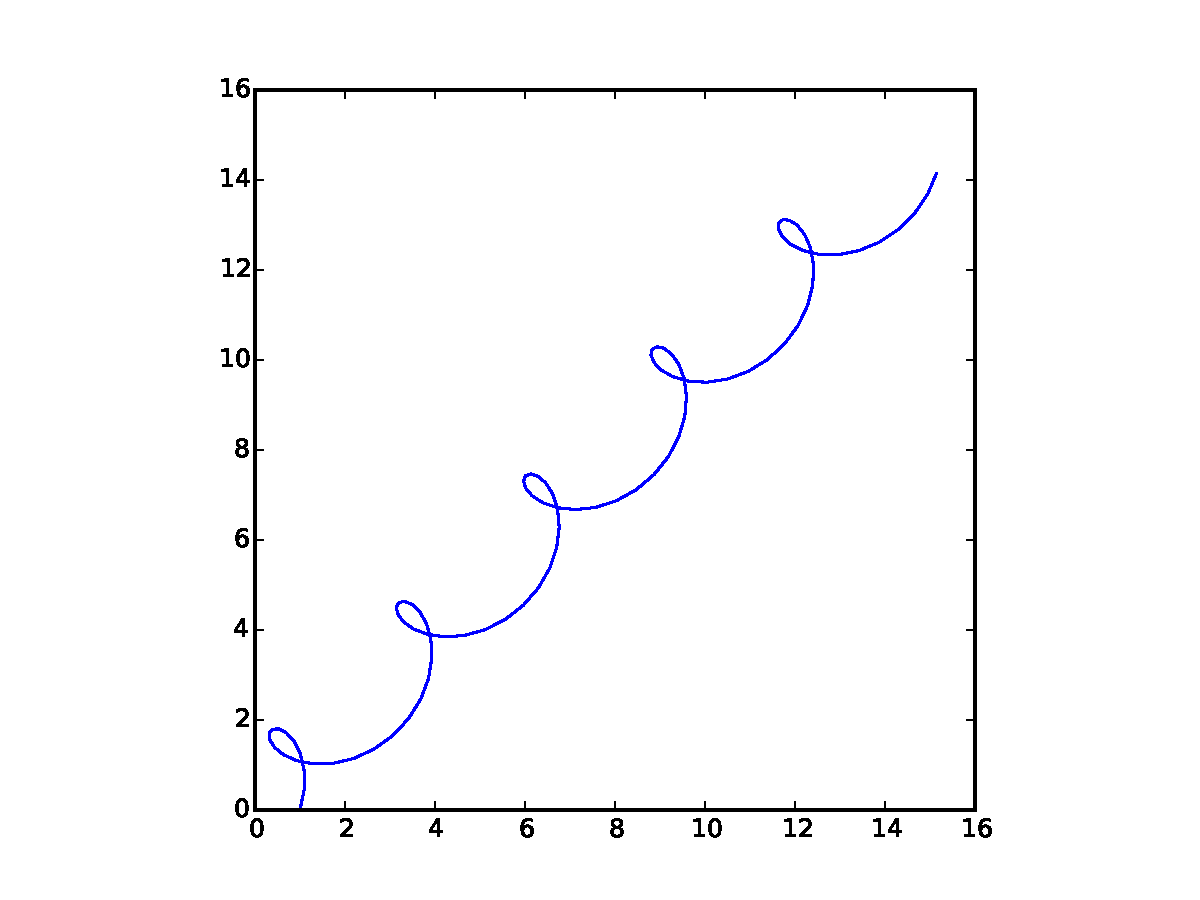
\includegraphics[width=\textwidth]{trajectory.pdf}
\caption{Solution to Problem \ref{prob:trajectory}.}
\label{fig:trajectory} 
\end{figure}
\end{problem}
